\section{Qsim::VmQMagic Struct Reference}
\label{structQsim_1_1VmQMagic}\index{Qsim::VmQMagic@{Qsim::VmQMagic}}
{\tt \#include $<$qsim.h$>$}

Inheritance diagram for Qsim::VmQMagic:\nopagebreak
\begin{figure}[H]
\begin{center}
\leavevmode
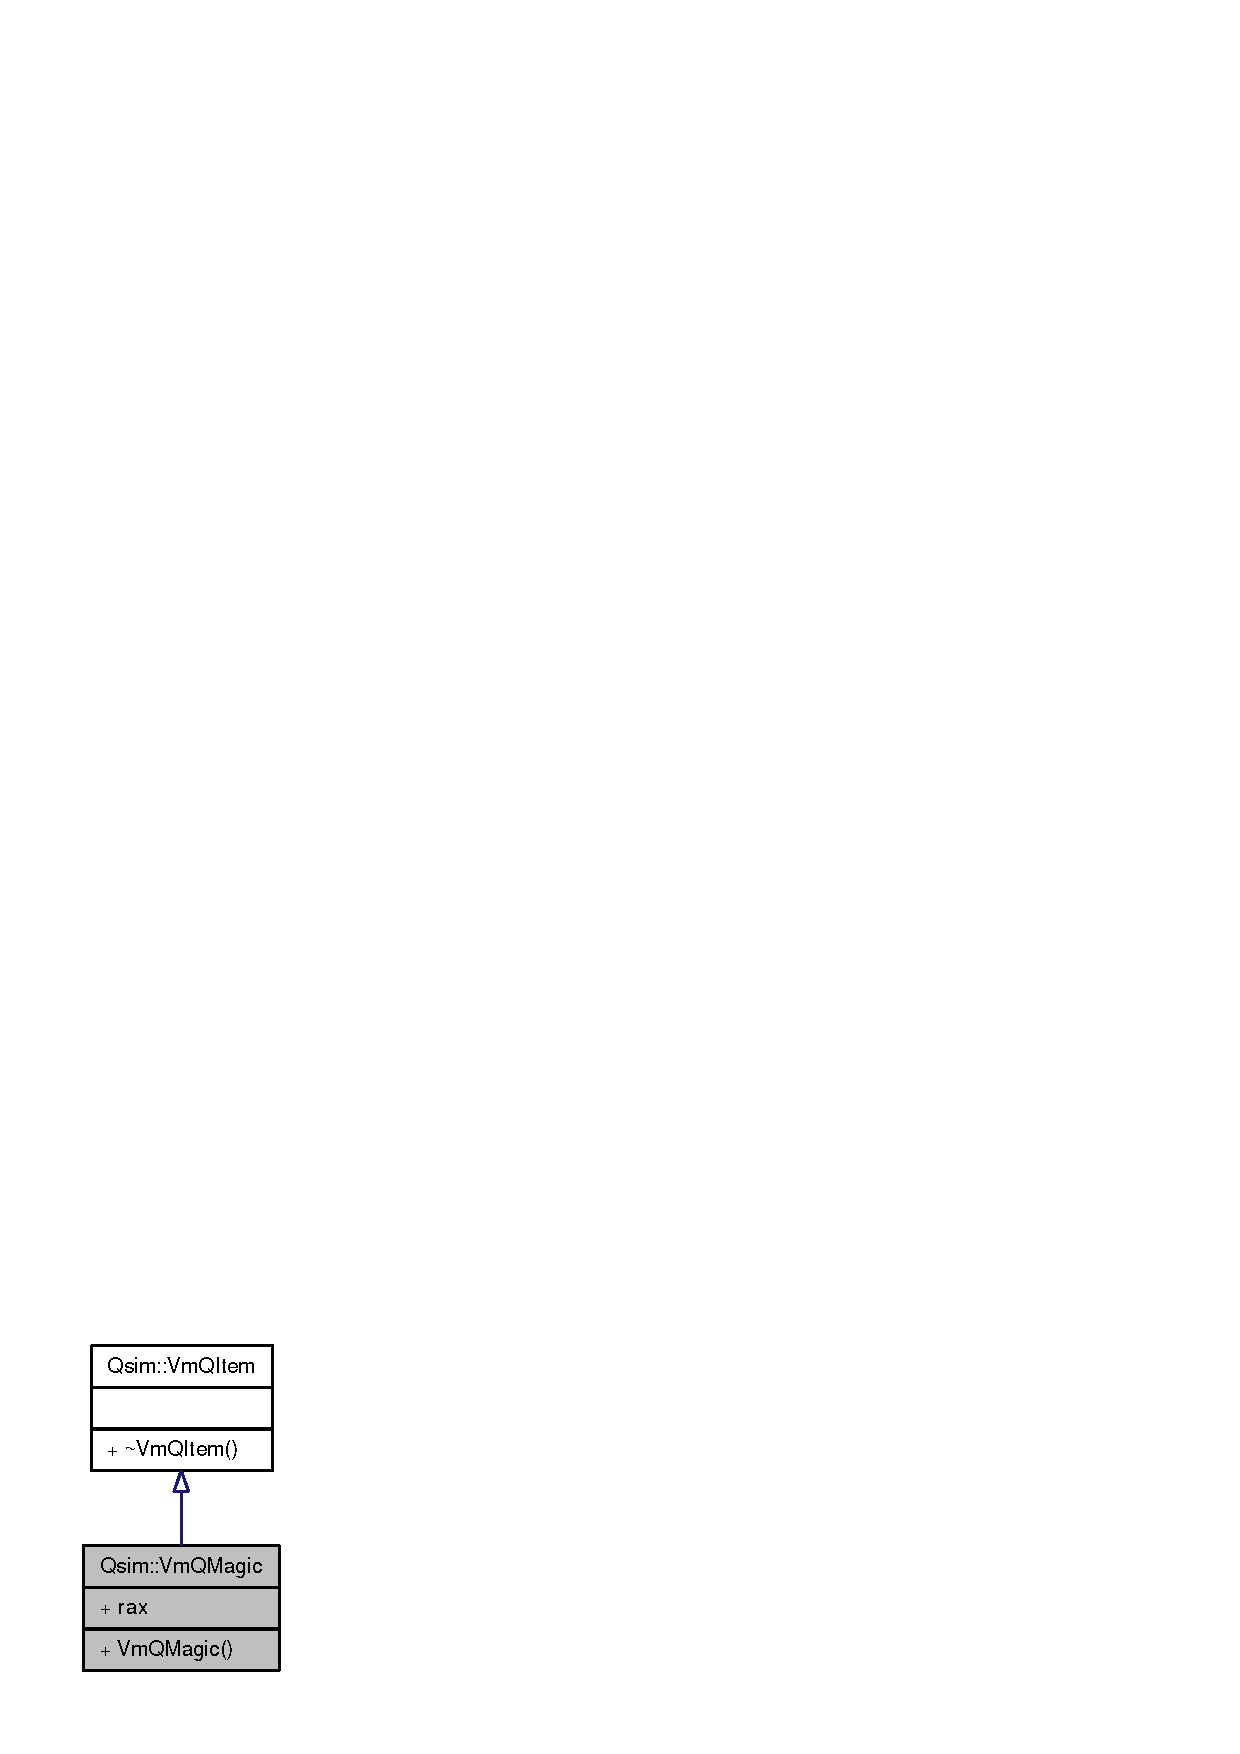
\includegraphics[width=138pt]{structQsim_1_1VmQMagic__inherit__graph}
\end{center}
\end{figure}
Collaboration diagram for Qsim::VmQMagic:\nopagebreak
\begin{figure}[H]
\begin{center}
\leavevmode
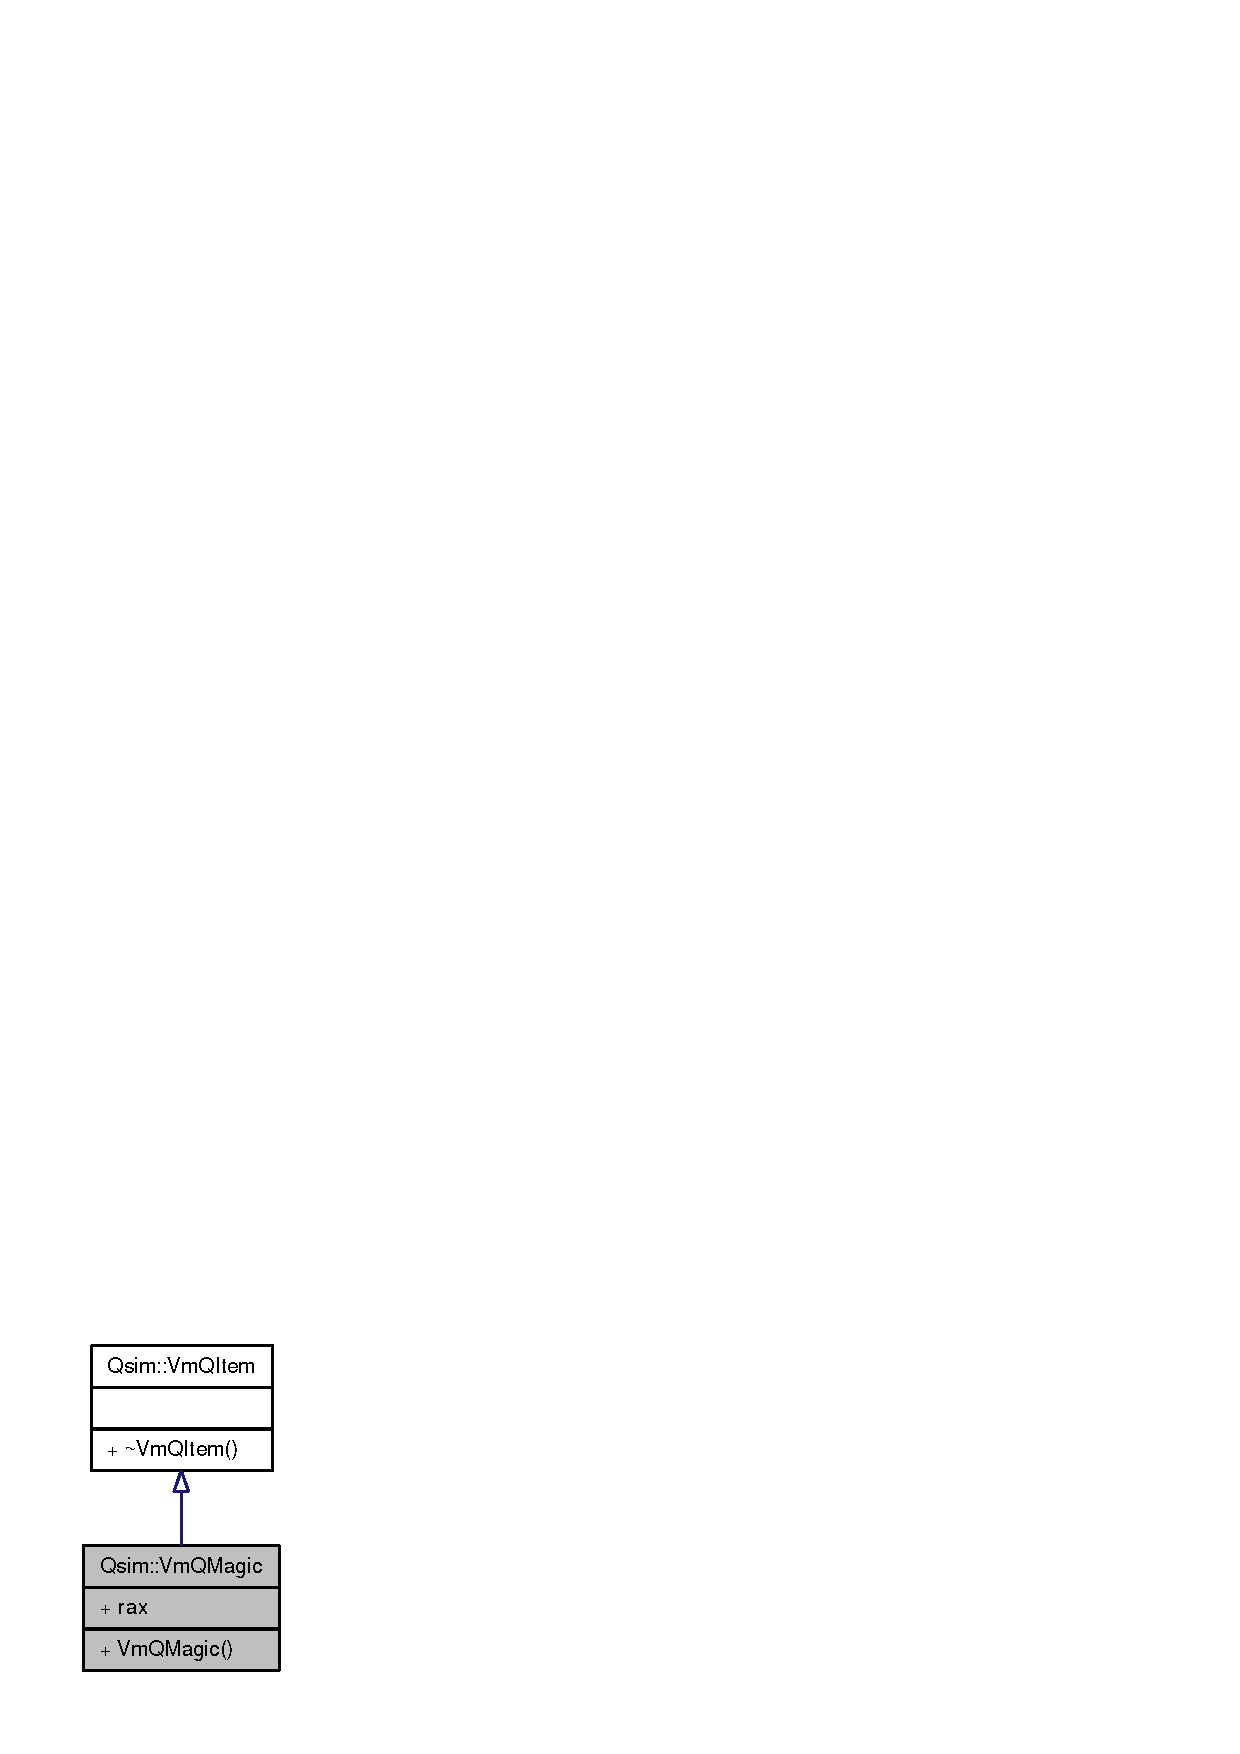
\includegraphics[width=138pt]{structQsim_1_1VmQMagic__coll__graph}
\end{center}
\end{figure}
\subsection*{Public Member Functions}
\begin{CompactItemize}
\item 
{\bf VmQMagic} (uint64\_\-t {\bf rax})
\end{CompactItemize}
\subsection*{Public Attributes}
\begin{CompactItemize}
\item 
uint64\_\-t {\bf rax}
\end{CompactItemize}


\subsection{Detailed Description}


Definition at line 114 of file qsim.h.

\subsection{Constructor \& Destructor Documentation}
\index{Qsim::VmQMagic@{Qsim::VmQMagic}!VmQMagic@{VmQMagic}}
\index{VmQMagic@{VmQMagic}!Qsim::VmQMagic@{Qsim::VmQMagic}}
\subsubsection[{VmQMagic}]{\setlength{\rightskip}{0pt plus 5cm}Qsim::VmQMagic::VmQMagic (uint64\_\-t {\em rax})\hspace{0.3cm}{\tt  [inline]}}\label{structQsim_1_1VmQMagic_f1b7480c9f5851f5d627180ee2178e33}




Definition at line 115 of file qsim.h.

\subsection{Member Data Documentation}
\index{Qsim::VmQMagic@{Qsim::VmQMagic}!rax@{rax}}
\index{rax@{rax}!Qsim::VmQMagic@{Qsim::VmQMagic}}
\subsubsection[{rax}]{\setlength{\rightskip}{0pt plus 5cm}uint64\_\-t {\bf Qsim::VmQMagic::rax}}\label{structQsim_1_1VmQMagic_a4865a01758678087e66d31c5c02f776}




Definition at line 116 of file qsim.h.

The documentation for this struct was generated from the following file:\begin{CompactItemize}
\item 
{\bf qsim.h}\end{CompactItemize}
